% modelo beamer
% http://latexbr.blogspot.com.br/
% aspectratio=169 - modo widescreen
\documentclass[aspectratio=169,mathserif]{beamer}
\usepackage[utf8]{inputenc}
\usepackage[T1]{fontenc}
\usepackage[english]{babel}
\usepackage{graphics,amssymb,amsfonts,amsmath}

\usepackage{algorithm,algpseudocode}
\usepackage{indentfirst}

\usepackage[skip=-2pt]{caption}
%\captionsetup{font={stretch=0.6,small}}

\usepackage{graphicx}
\usepackage{subfig}
\usepackage{array,multirow}
%\usepackage{listings}
\usepackage{tikz}
\usepackage{color}
\usepackage{enumerate,hyperref}
%\usepackage{palatino}	% Fonte sem serifa
\usepackage{ragged2e}	% Paragrafo justificado
%\usepackage{minted}	% Highlight para codigos de programacao
\usepackage{booktabs} % tabelas
\usepackage[round,sort]{natbib}
%\usepackage{lipsum}
\usepackage{tcolorbox}
\usepackage{verbatim}
%\usepackage[alf]{abntex2cite}
\usepackage{float}
%\usepackage{subcaption}

\algnewcommand\algorithmicinput{\textbf{Input:}}
\algnewcommand\INPUT{\item[\algorithmicinput]}

\algnewcommand\algorithmicoutput{\textbf{Output:}}
\algnewcommand\OUTPUT{\item[\algorithmicoutput]}

\usetheme[height=7mm]{Rochester}
\setbeamertemplate{items}[default]
\setbeamertemplate{blocks}[rounded][shadow=true]
\setbeamertemplate{navigation symbols}{}
\AtBeginSection[]{\frame{\frametitle{Outline}\tableofcontents[current]}}


%\usetheme{Pittsburgh}
\usecolortheme{orchid}
\usefonttheme[onlymath]{serif}
%\usepackage{multimedia}
\usepackage[3D]{movie15} % adiciona esse pacote no preâmbulo
\usepackage[labelformat=empty]{caption}
\definecolor{mygreen}  {HTML}{A0C307}
\definecolor{mygreen2} {HTML}{E5F694}
\definecolor{myblue}   {HTML}{37ADC9}
\definecolor{myblue2}  {HTML}{B9D9E1}
\definecolor{myorange} {HTML}{FF8110}
\definecolor{myorange2}{HTML}{FFCC67}
\definecolor{mypink}   {HTML}{FF4B9C}
\definecolor{mypink2}  {HTML}{FFC5DF}
\definecolor{darkgreen}  {HTML}{008000}
\usepackage{pgfkeys}
\usepackage{tikz}

% Colocando numero de paginas no slide
\setbeamertemplate{footline}[frame number]

% Desativando os botoes de navegacao
\beamertemplatenavigationsymbolsempty


% Tela cheia
%\hypersetup{pdfpagemode=FullScreen}

% Layout da pagina
\hypersetup{pdfpagelayout=SinglePage}

% Definicao de novos ambientes
%\theoremstyle{Definition}
\newtheorem{definicao}{Defini\c c\~ao}
\newtheorem{exemplo}{Exemplo}
\newtheorem{proposicao}{Proposição}
\newtheorem{teo}[theorem]{Teorema}
\newcommand{\xbf}{\boldsymbol{x}}
\newcommand{\ybf}{\boldsymbol{y}}
% Definicao de novos comandos
\providecommand{\sin}{} \renewcommand{\sin}{\hspace{2pt}\textrm{sen}}
\providecommand{\tan}{} \renewcommand{\tan}{\hspace{2pt}\textrm{tg}}
\newcommand{\R}{\mathbb{R}}
\newcommand{\betabf}{\boldsymbol{\beta}}
\newcommand{\I}{\textbf{I}}
\newcommand{\K}{\textbf{k}}
\newcommand{\sen}{\mathrm{\ sen}}
% Capa - requer o TikZ
\newcommand{\capa}{
  \begin{tikzpicture}[remember picture,overlay]
    \node at (current page.south west);
      %{\begin{tikzpicture}[remember picture, overlay]
        \fill[shading=radial,top color=blue,bottom color=white,middle color=white]
          (0,0) rectangle (\paperwidth,\paperheight);
      %\end{tikzpicture}
      %}
  \end{tikzpicture}
}

\setbeamersize{text margin left=10pt,text margin right=10pt}

% Titulo

\title[\sc{footnote}]{Constructive and Local Search Heuristics \vspace{0.2cm} \\ for the Splitwise Problem}
\author[]{
    \textbf{\color{orange} Filipe Gomes Arante de Souza}\\
}

\date{Metaheuristics 2026/2, UFES, September, 2026}
\institute[]{filipe.gomes.arante@gmail.com} % opcional


% \institute{Universidade Federal do Espírito Santo} % opcional
%\date{}

% ==============================================================================
% Formatação do Slide de Capa
% ==============================================================================
\pgfdeclareimage[width=\paperwidth]{planodefundo}{Figuras/capa}
\setbeamerfont{subtitle}{size=\scriptsize}
\setbeamertemplate{title page}{
\begin{picture}(0,0)
  \put(-28.5,-153){%
    \pgfuseimage{planodefundo}
  }
  \put(0,-75){%
    \begin{minipage}[b][4.5cm][t]{0.75\textwidth}
    \color{white}
    \usebeamerfont{title}
      {{\color{white}\large\textbf{\inserttitle}}\\[0.2cm]}
      {{\color{white}\normalsize\textbf{\insertsubtitle}}\\[1.5cm]}
    \usebeamerfont{subtitle}
      {\insertauthor\\[0.5cm]}
      {\insertinstitute\\[0.3cm]}
      {\tiny{\insertdate}}
  \end{minipage}
  }
\end{picture}
}

\begin{document}

\begin{frame}[plain]
    \titlepage
\end{frame}

\part{Main Part}
\frame{\frametitle{Outline}\tableofcontents[part=1]}

\section{Splitwise Problem}

\begin{frame}
    \frametitle{Splitwise Problem}
    \begin{block}{Definition}
        Given a set of $n$ people and a balance vector $B = (b_1, ..., b_n)$, where $b_i > 0$ means person $i$ should receive money, $b_i < 0$ means person $i$ owes money, and $b_i = 0$ means no transaction is needed for that person, with $\sum_{i=0}^{n} b_i = 0$, the objective is to find the minimum number of transactions $(i, j, v)$, where person $i$ pays $v$ units to person $j$ such that everyone ends up settled.
    \end{block}
\end{frame}

% \begin{frame}
%    \frametitle{Example with figure}
%    \begin{figure}
%        \centering
%        \includegraphics[height=3.8cm, width=6cm]{Figuras/Menezes2017.eps}
%        \caption{\tiny{{\bf Source:} Menezes et al. A branch and price algorithm to solve the integrated production  planning and scheduling in bulk ports, European Journal of Operational Research, 2017.}}
%    \end{figure}
% \end{frame}

\section{Greedy Constructive Algorithm}

\foreach \n in {1,...,8} {
        \begin{frame}{Greedy Constructive Algorithm}
            \centering
            \includegraphics[width=\textwidth]{images/step_by_step_greedy/greedy_0\n.eps}
        \end{frame}
    }

\begin{frame}
    \frametitle{Greedy Constructive Algorithm}
    \begin{itemize}
        \item People with \textbf{exactly opposite balances} are paired off directly (one transaction each)
        \item The rest are settled by repeatedly matching the \textbf{largest debtor against the largest creditor}
        \item Each match cancels at least one side's balance completely, so it never revisits a settled person
    \end{itemize}
\end{frame}

\begin{frame}{Greedy Constructive Algorithm}
    \begin{columns}
        \column{0.02\textwidth}
        \column{0.98\textwidth}
        \footnotesize{\begin{algorithmic}[1]
    \INPUT  Balances vector $b[1..n]$, indexed by person, with $\sum_{p=1}^{n} b[p] = 0$.
    \OUTPUT Set of transactions $T$.

    \State $(T_{\text{pairs}}, L) \leftarrow \texttt{PairExactMatches}(b)$ \Comment{$L$: people left with a nonzero balance}
    \State $T \leftarrow T_{\text{pairs}}$

    \State $\textit{Debtors} \leftarrow \{p \in L : b[p] < 0\}$, $\textit{Creditors} \leftarrow \{p \in L : b[p] > 0\}$

    \While{$\textit{Debtors} \neq \emptyset$ \textbf{and} $\textit{Creditors} \neq \emptyset$}
        \State $debtor \leftarrow \arg\max_{p \in \textit{Debtors}} (-b[p])$
        \State $creditor \leftarrow \arg\max_{p \in \textit{Creditors}} (b[p])$
        \State $amount \leftarrow \min(-b[debtor],\, b[creditor])$

        \State $T \leftarrow T \cup \{(debtor, creditor, amount)\}$
        \State $b[debtor] \leftarrow b[debtor] + amount$
        \State $b[creditor] \leftarrow b[creditor] - amount$

        \If{$b[debtor] = 0$}
            \State $\textit{Debtors} \leftarrow \textit{Debtors} \setminus \{debtor\}$
        \EndIf
        \If{$b[creditor] = 0$}
            \State $\textit{Creditors} \leftarrow \textit{Creditors} \setminus \{creditor\}$
        \EndIf
    \EndWhile

    \State \Return $T$

\end{algorithmic}}
    \end{columns}
\end{frame}


\section {Random Keys Based Constructive Algorithm}

\foreach \n in {1,...,13} {
        \begin{frame}{Random Keys Based Constructive Algorithm}
            \centering
            \includegraphics[width=\textwidth]{images/step_by_step_random_keys/rk_\n.eps}
        \end{frame}
    }

\begin{frame} \frametitle{Random Keys Based Constructive Algorithm}
    \begin{itemize}
        \item Each person gets a \textbf{random key} (a number in $[0,1]$)
        \item People are \textbf{sorted} by their key $\rightarrow$ produces a random permutation $\pi$
        \item $\pi$ is scanned and partitioned into \textbf{zero-sum groups} via running partial sums
        \item Each group is \textbf{settled independently} by the greedy method
    \end{itemize}
\end{frame}

\begin{frame}{Random Keys Based Constructive Algorithm}
    \begin{columns}
        \column{0.02\textwidth}
        \column{0.98\textwidth}
        \footnotesize{\begin{algorithmic}[1]
    \INPUT  Balances vector $b[1..n]$, indexed by person, with $\sum_{p=1}^{n} b[p] = 0$.
    \OUTPUT Set of transactions $T$.

    \State $(T_{\text{pairs}}, L) \leftarrow \texttt{PairExactMatches}(b)$ \Comment{$L$: people left with a nonzero balance}
    \State $T \leftarrow T_{\text{pairs}}$

    \State draw $r[p] \sim U(0,1)$ for each $p \in L$
    \State $\pi \leftarrow$ sort $L$ by $r[p]$, ascending

    \State $\mathcal{G} \leftarrow \texttt{ZeroSumGroups}(\pi, b)$ \Comment{partition $\pi$ into disjoint groups, each summing to zero}

    \ForAll{$g \in \mathcal{G}$}
    \State $T \leftarrow T \cup \texttt{Greedy}(g, b)$
    \EndFor

    \State \Return $T$

\end{algorithmic}}
    \end{columns}
\end{frame}

\section{Local Search}

\begin{frame}{Local Search}
    \begin{itemize}
        \item Starts from a solution and its respective order $\pi$
        \item The neighborhood is every \textbf{swap of two people's positions} in $\pi$
        \item Movements are \textbf{performed into $\pi$}
        \item Neighbor solutions are computed using \textbf{random key constructive algorithm}
    \end{itemize}
\end{frame}

\begin{frame}{Best Improvement}
    \begin{columns}
        \column{0.02\textwidth}
        \column{0.98\textwidth}
        \footnotesize{\begin{algorithmic}[1]
    \INPUT  Set of transactions $T$, order $\pi = (\pi_1, \dots, \pi_n)$ of the people, balances vector $b[1..n]$.
    \OUTPUT Locally optimal set of transactions $T^\star$ and its order $\pi^\star$.

    \State $T^\star \leftarrow T$
    \State $\pi^\star \leftarrow \pi$
    \State $\textit{improved} \leftarrow \textbf{true}$

    \While{\textit{improved}}
        \State $\textit{improved} \leftarrow \textbf{false}$

        \For{$i \leftarrow 1$ \textbf{to} $n - 1$}
            \For{$j \leftarrow i + 1$ \textbf{to} $n$}
                \State $\pi' \leftarrow \texttt{Swap}(\pi^\star, i, j)$
                \State $T' \leftarrow \texttt{Decode}(\pi', b)$

                \If{$f(T') < f(T^\star)$}
                    \State $T^\star \leftarrow T'$
                    \State $\pi^\star \leftarrow \pi'$
                    \State $\textit{improved} \leftarrow \textbf{true}$
                \EndIf
            \EndFor
        \EndFor
    \EndWhile

    \State \Return $(T^\star, \pi^\star)$

\end{algorithmic}}
    \end{columns}
\end{frame}

\begin{frame}{First Improvement}
    \begin{columns}
        \column{0.02\textwidth}
        \column{0.98\textwidth}
        \footnotesize{\begin{algorithmic}[1]
    \INPUT  Set of transactions $T$, order $\pi = (\pi_1, \dots, \pi_n)$ of the people, balances vector $b[1..n]$.
    \OUTPUT Locally optimal set of transactions $T^\star$ and its order $\pi^\star$.

    \State $T^\star \leftarrow T$, $\pi^\star \leftarrow \pi$, $\textit{improved} \leftarrow \textbf{true}$

    \While{\textit{improved}}
        \State $\textit{improved} \leftarrow \textbf{false}$

        \For{$i \leftarrow 1$ \textbf{to} $n - 1$}
            \For{$j \leftarrow i + 1$ \textbf{to} $n$}
                \State $\pi' \leftarrow \texttt{Swap}(\pi^\star, i, j)$
                \State $T' \leftarrow \texttt{Decode}(\pi', b)$

                \If{$f(T') < f(T^\star)$}
                    \State $T^\star \leftarrow T'$, $\pi^\star \leftarrow \pi'$, $\textit{improved} \leftarrow \textbf{true}$
                    \State \textbf{break}
                \EndIf
            \EndFor

            \If{\textit{improved}}
                \State \textbf{break}
            \EndIf
        \EndFor
    \EndWhile

    \State \Return $(T^\star, \pi^\star)$

\end{algorithmic}}
    \end{columns}
\end{frame}

\section{Experiments}

\begin{frame}{Experiments}
    \begin{block}{Instances}
        $32$ instances with balances from $20$ to $1500$ people. Each of them contains several subsets with sum $0$ and were built by the students in the course.
    \end{block}
\end{frame}

\begin{frame}{Experiments}
    \begin{itemize}
        \item Instances with sizes ranging from $20$ to $900$ were run on a Google Colaboratory environment, to allow comparison between the students implementations.
        \item Instances with size over $900$ were run on a computer equipped with an AMD Ryzen 7 9700X processor running at 3.8GHz (5.5GHz Turbo), 32GB 6000MHz RAM, and the Ubuntu 24.04 operating system for deadline reasons.
        \item All source code was implemented in Python 3.12.3.
    \end{itemize}
\end{frame}

\section{Results}

\begin{frame}{Results}
    \begin{table}[h]
\centering
\resizebox{\textwidth}{!}{%
\begin{tabular}{|l|rr|rr|rrr|rrr|rrr|rrr|}
\hline
\multirow{2}{*}{$Instance$} & \multicolumn{2}{c|}{$AC_G$} & \multicolumn{2}{c|}{$AC_R$} &
\multicolumn{3}{c|}{$BL_{FI}(AC_G)$} & \multicolumn{3}{c|}{$BL_{FI}(AC_R)$} &
\multicolumn{3}{c|}{$BL_{BI}(AC_G)$} & \multicolumn{3}{c|}{$BL_{BI}(AC_R)$} \\
\cline{2-17}
 & $sol$ & $t(s)$ & $sol$ & $t(s)$
 & $sol$ & $N_{It}$ & $t(s)$ & $sol$ & $N_{It}$ & $t(s)$
 & $sol$ & $N_{It}$ & $t(s)$ & $sol$ & $N_{It}$ & $t(s)$ \\
\hline
20 & 17 & 0.001 & 16 & 0.000 & \textbf{15} & 3 & 0.003 & \textbf{15} & 2 & 0.003 & \textbf{15} & 2 & 0.004 & \textbf{15} & 2 & 0.005 \\
30 & 23 & 0.000 & 23 & 0.000 & \textbf{22} & 2 & 0.013 & \textbf{22} & 2 & 0.013 & \textbf{22} & 2 & 0.014 & \textbf{22} & 2 & 0.017 \\
30\_5 & 27 & 0.000 & 27 & 0.001 & \textbf{26} & 2 & 0.016 & \textbf{26} & 2 & 0.017 & \textbf{26} & 2 & 0.029 & \textbf{26} & 2 & 0.035 \\
50 & 39 & 0.000 & 40 & 0.000 & \textbf{36} & 4 & 0.047 & \textbf{36} & 4 & 0.051 & \textbf{36} & 4 & 0.125 & \textbf{36} & 4 & 0.128 \\
50\_8 & 40 & 0.000 & 41 & 0.000 & 38 & 3 & 0.028 & 36 & 6 & 0.041 & \textbf{35} & 4 & 0.088 & \textbf{35} & 4 & 0.089 \\
100 & 77 & 0.000 & 79 & 0.001 & \textbf{74} & 4 & 0.759 & 75 & 5 & 0.350 & \textbf{74} & 4 & 1.107 & \textbf{74} & 4 & 1.042 \\
100\_20 & 74 & 0.001 & 73 & 0.001 & \textbf{68} & 6 & 0.112 & \textbf{68} & 5 & 0.191 & \textbf{68} & 3 & 0.279 & \textbf{68} & 3 & 0.271 \\
150 & 119 & 0.001 & 121 & 0.001 & 110 & 10 & 2.059 & 111 & 11 & 1.274 & \textbf{109} & 7 & 6.568 & \textbf{109} & 7 & 6.031 \\
150\_15 & 147 & 0.001 & 147 & 0.001 & \textbf{143} & 5 & 1.938 & \textbf{143} & 5 & 1.939 & \textbf{143} & 2 & 1.525 & \textbf{143} & 2 & 1.546 \\
200 & 159 & 0.001 & 164 & 0.001 & \textbf{148} & 12 & 6.392 & 149 & 13 & 6.136 & \textbf{148} & 8 & 13.877 & \textbf{148} & 8 & 14.081 \\
200\_8 & 136 & 0.001 & 138 & 0.001 & 131 & 4 & 3.261 & \textbf{130} & 8 & 2.903 & 131 & 4 & 5.579 & 131 & 4 & 4.378 \\
200\_80 & 144 & 0.000 & 144 & 0.001 & 140 & 3 & 0.324 & 140 & 3 & 0.596 & \textbf{137} & 4 & 1.490 & \textbf{137} & 4 & 1.702 \\
300 & 240 & 0.001 & 239 & 0.001 & 222 & 18 & 28.311 & \textbf{221} & 18 & 35.799 & 224 & 8 & 45.870 & 224 & 8 & 46.392 \\
300\_60 & 248 & 0.001 & 241 & 0.001 & 227 & 12 & 17.407 & \textbf{224} & 12 & 15.398 & 227 & 5 & 31.543 & 227 & 5 & 32.154 \\
400 & 312 & 0.001 & 313 & 0.001 & 294 & 18 & 67.823 & 293 & 21 & 120.810 & \textbf{291} & 13 & 181.495 & \textbf{291} & 13 & 181.818 \\
400\_35 & 317 & 0.001 & 305 & 0.002 & \textbf{290} & 11 & 33.096 & 295 & 8 & 36.508 & 294 & 4 & 45.472 & 294 & 4 & 46.345 \\
\hline
\end{tabular}%
}
\label{tab:resultados-parte1}
\end{table}
\end{frame}

\begin{frame}{Results}
    \begin{table}[h]
\centering
\resizebox{\textwidth}{!}{%
\begin{tabular}{|l|rr|rr|rrr|rrr|rrr|rrr|}
\hline
\multirow{2}{*}{$Instance$} & \multicolumn{2}{c|}{$AC_G$} & \multicolumn{2}{c|}{$AC_R$} &
\multicolumn{3}{c|}{$BL_{FI}(AC_G)$} & \multicolumn{3}{c|}{$BL_{FI}(AC_R)$} &
\multicolumn{3}{c|}{$BL_{BI}(AC_G)$} & \multicolumn{3}{c|}{$BL_{BI}(AC_R)$} \\
\cline{2-17}
 & $sol$ & $t(s)$ & $sol$ & $t(s)$
 & $sol$ & $N_{It}$ & $t(s)$ & $sol$ & $N_{It}$ & $t(s)$
 & $sol$ & $N_{It}$ & $t(s)$ & $sol$ & $N_{It}$ & $t(s)$ \\
\hline
500 & 391 & 0.001 & 395 & 0.002 & 370 & 21 & 182.382 & \textbf{365} & 29 & 271.455 & 367 & 16 & 438.512 & 367 & 16 & 435.920 \\
500\_188 & 290 & 0.001 & 296 & 0.001 & 286 & 4 & 2.006 & \textbf{284} & 9 & 1.625 & \textbf{284} & 4 & 5.162 & \textbf{284} & 4 & 4.524 \\
500\_25 & 349 & 0.001 & 356 & 0.004 & \textbf{339} & 10 & 85.440 & 341 & 13 & 55.946 & 341 & 5 & 113.511 & 341 & 5 & 104.829 \\
600 & 481 & 0.001 & 473 & 0.002 & 440 & 31 & 589.130 & 440 & 31 & 589.176 & \textbf{438} & 20 & 937.882 & \textbf{438} & 20 & 939.644 \\
600\_40 & 312 & 0.001 & 315 & 0.001 & 312 & 1 & 0.128 & \textbf{311} & 5 & 0.198 & 312 & 1 & 0.111 & 312 & 3 & 0.334 \\
700 & 555 & 0.001 & 549 & 0.002 & 513 & 36 & 1277.535 & 514 & 36 & 1267.302 & \textbf{511} & 18 & 1343.988 & \textbf{511} & 18 & 1352.447 \\
700\_90 & 509 & 0.003 & 517 & 0.004 & 479 & 11 & 99.968 & 483 & 15 & 236.067 & \textbf{477} & 8 & 552.971 & \textbf{477} & 8 & 558.702 \\
800 & 637 & 0.002 & 644 & 0.004 & 584 & 51 & 2189.409 & \textbf{581} & 59 & 2647.648 & 587 & 23 & 2500.286 & 587 & 23 & 2493.053 \\
800\_80 & 575 & 0.002 & 582 & 0.004 & \textbf{539} & 19 & 403.217 & 542 & 23 & 335.636 & 543 & 5 & 450.940 & 543 & 5 & 453.984 \\
900 & 706 & 0.002 & 713 & 0.003 & \textbf{658} & 44 & 3690.089 & 661 & 49 & 2757.153 & 662 & 23 & 3502.355 & 662 & 23 & 3488.820 \\
900\_100 & 542 & 0.003 & 549 & 0.003 & \textbf{529} & 13 & 85.290 & \textbf{529} & 17 & 67.474 & \textbf{529} & 8 & 123.833 & \textbf{529} & 8 & 121.863 \\
1000 & 797 & 0.001 & 795 & 0.001 & \textbf{731} & 62 & 986.569 & \textbf{731} & 56 & 1138.474 & 732 & 27 & 1288.976 & 732 & 27 & 1311.561 \\
1000\_120 & 559 & 0.001 & 560 & 0.002 & 550 & 10 & 3.343 & 554 & 6 & 0.990 & \textbf{549} & 6 & 3.771 & \textbf{549} & 6 & 3.780 \\
1100 & 870 & 0.001 & 867 & 0.001 & \textbf{803} & 55 & 1825.537 & 809 & 53 & 1656.228 & 810 & 28 & 1870.567 & 810 & 28 & 1873.492 \\
1300 & 1013 & 0.001 & 1038 & 0.001 & 1013 & 1 & 112.169 & 960 & 73 & 3177.233 & 1013 & 1 & 112.497 & \textbf{958} & 32 & 3437.296 \\
1500 & 1176 & 0.001 & 1191 & 0.001 & 1176 & 1 & 175.510 & \textbf{1098} & 89 & 4275.230 & 1176 & 1 & 174.197 & 1103 & 43 & 7244.611 \\
\hline
\end{tabular}%
}
\label{tab:resultados-parte2}
\end{table}
\end{frame}

\begin{frame}{Results}
    \begin{figure}
        \centering
        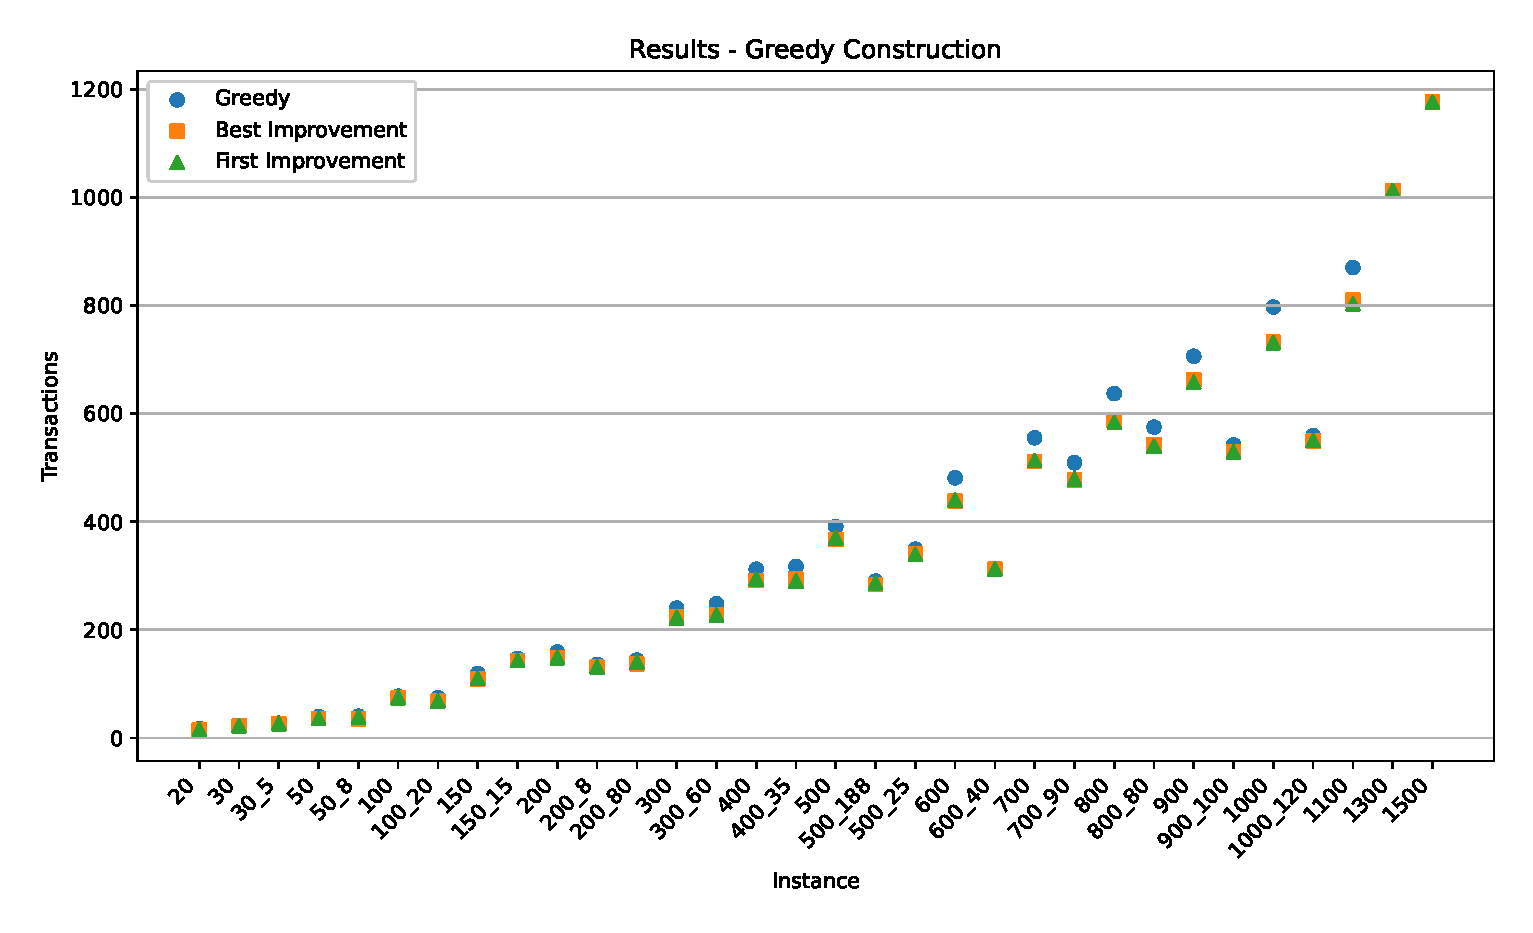
\includegraphics[width=0.8\textwidth]{graphics/fitness_greedy.eps}
    \end{figure}
\end{frame}

\begin{frame}{Results}
    \begin{figure}
        \centering
        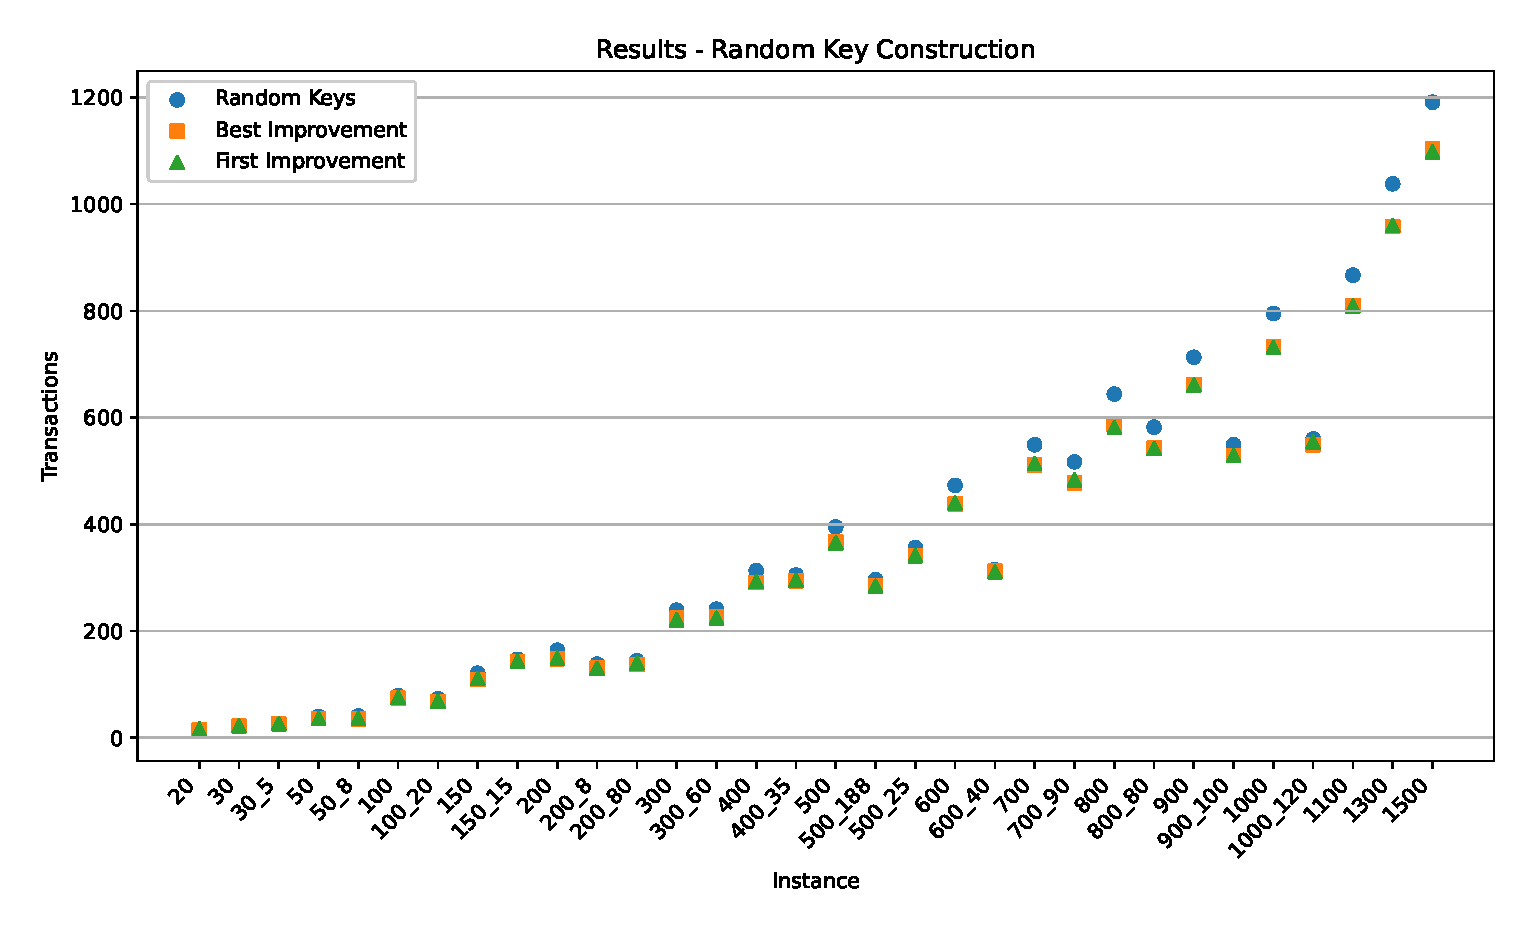
\includegraphics[width=0.8\textwidth]{graphics/fitness_random_key.eps}
    \end{figure}
\end{frame}

\section{Conclusions}

\begin{frame}{Conclusions about constructive algorithms}
    \begin{itemize}
        \item 19 victories for greedy approach
        \item 9 victories for random keys approach
        \item 4 ties
        \item 0.4\% relative gap
        \item Both are really fast, running in insignificant time
        \item \textbf{Obs:} random keys algorithm was executed just once. It would be interesting analyse its behavior in many runs
    \end{itemize}
\end{frame}

\begin{frame}{Conclusions about local searches}
    \begin{itemize}
        \item Starting from \textbf{greedy algorithm}: 10 victories for BI, 8 victories for FI and 14 ties
        \item Starting from \textbf{random key algorithm}: 12 victories for BI, 11 victories for FI and 9 ties
        \item \textbf{Random key + BI}: 13479s, 270 iterations
        \item \textbf{Random key + FI}: 11247s, 526 iterations
        \item \textbf{Greedy + BI}: 13468s, 268 iterations
        \item \textbf{Greedy + FI}: 11582s, 485 iterations
        \item Equivalent results, but \textbf{FI strategy is faster than BI strategy} and performs about \textbf{double the iterations}
        \item BI strategy obtained same result in all instances except two of them. The result \textbf{converges independently the initial solution}
    \end{itemize}
\end{frame}

\begin{frame}
    \begin{center}
        {\huge \bf \color{mypink} Thank you!} \\ \vspace{1cm}
        \begin{tabular}{cc}
            Filipe Gomes Arante de Souza               \\
            {\bf \small filipe.gomes.arante@gmail.com} \\
        \end{tabular}
    \end{center}
\end{frame}
\end{document}


